\chapter{Experiment 2}

\textbf{Author: } 


\section{Setup}
[TODO: viele Fotos]

\section{Environment}


\begin{figure*}[h!]
	\centering
	\begin{subfigure}[t]{\textwidth}
		\centering
		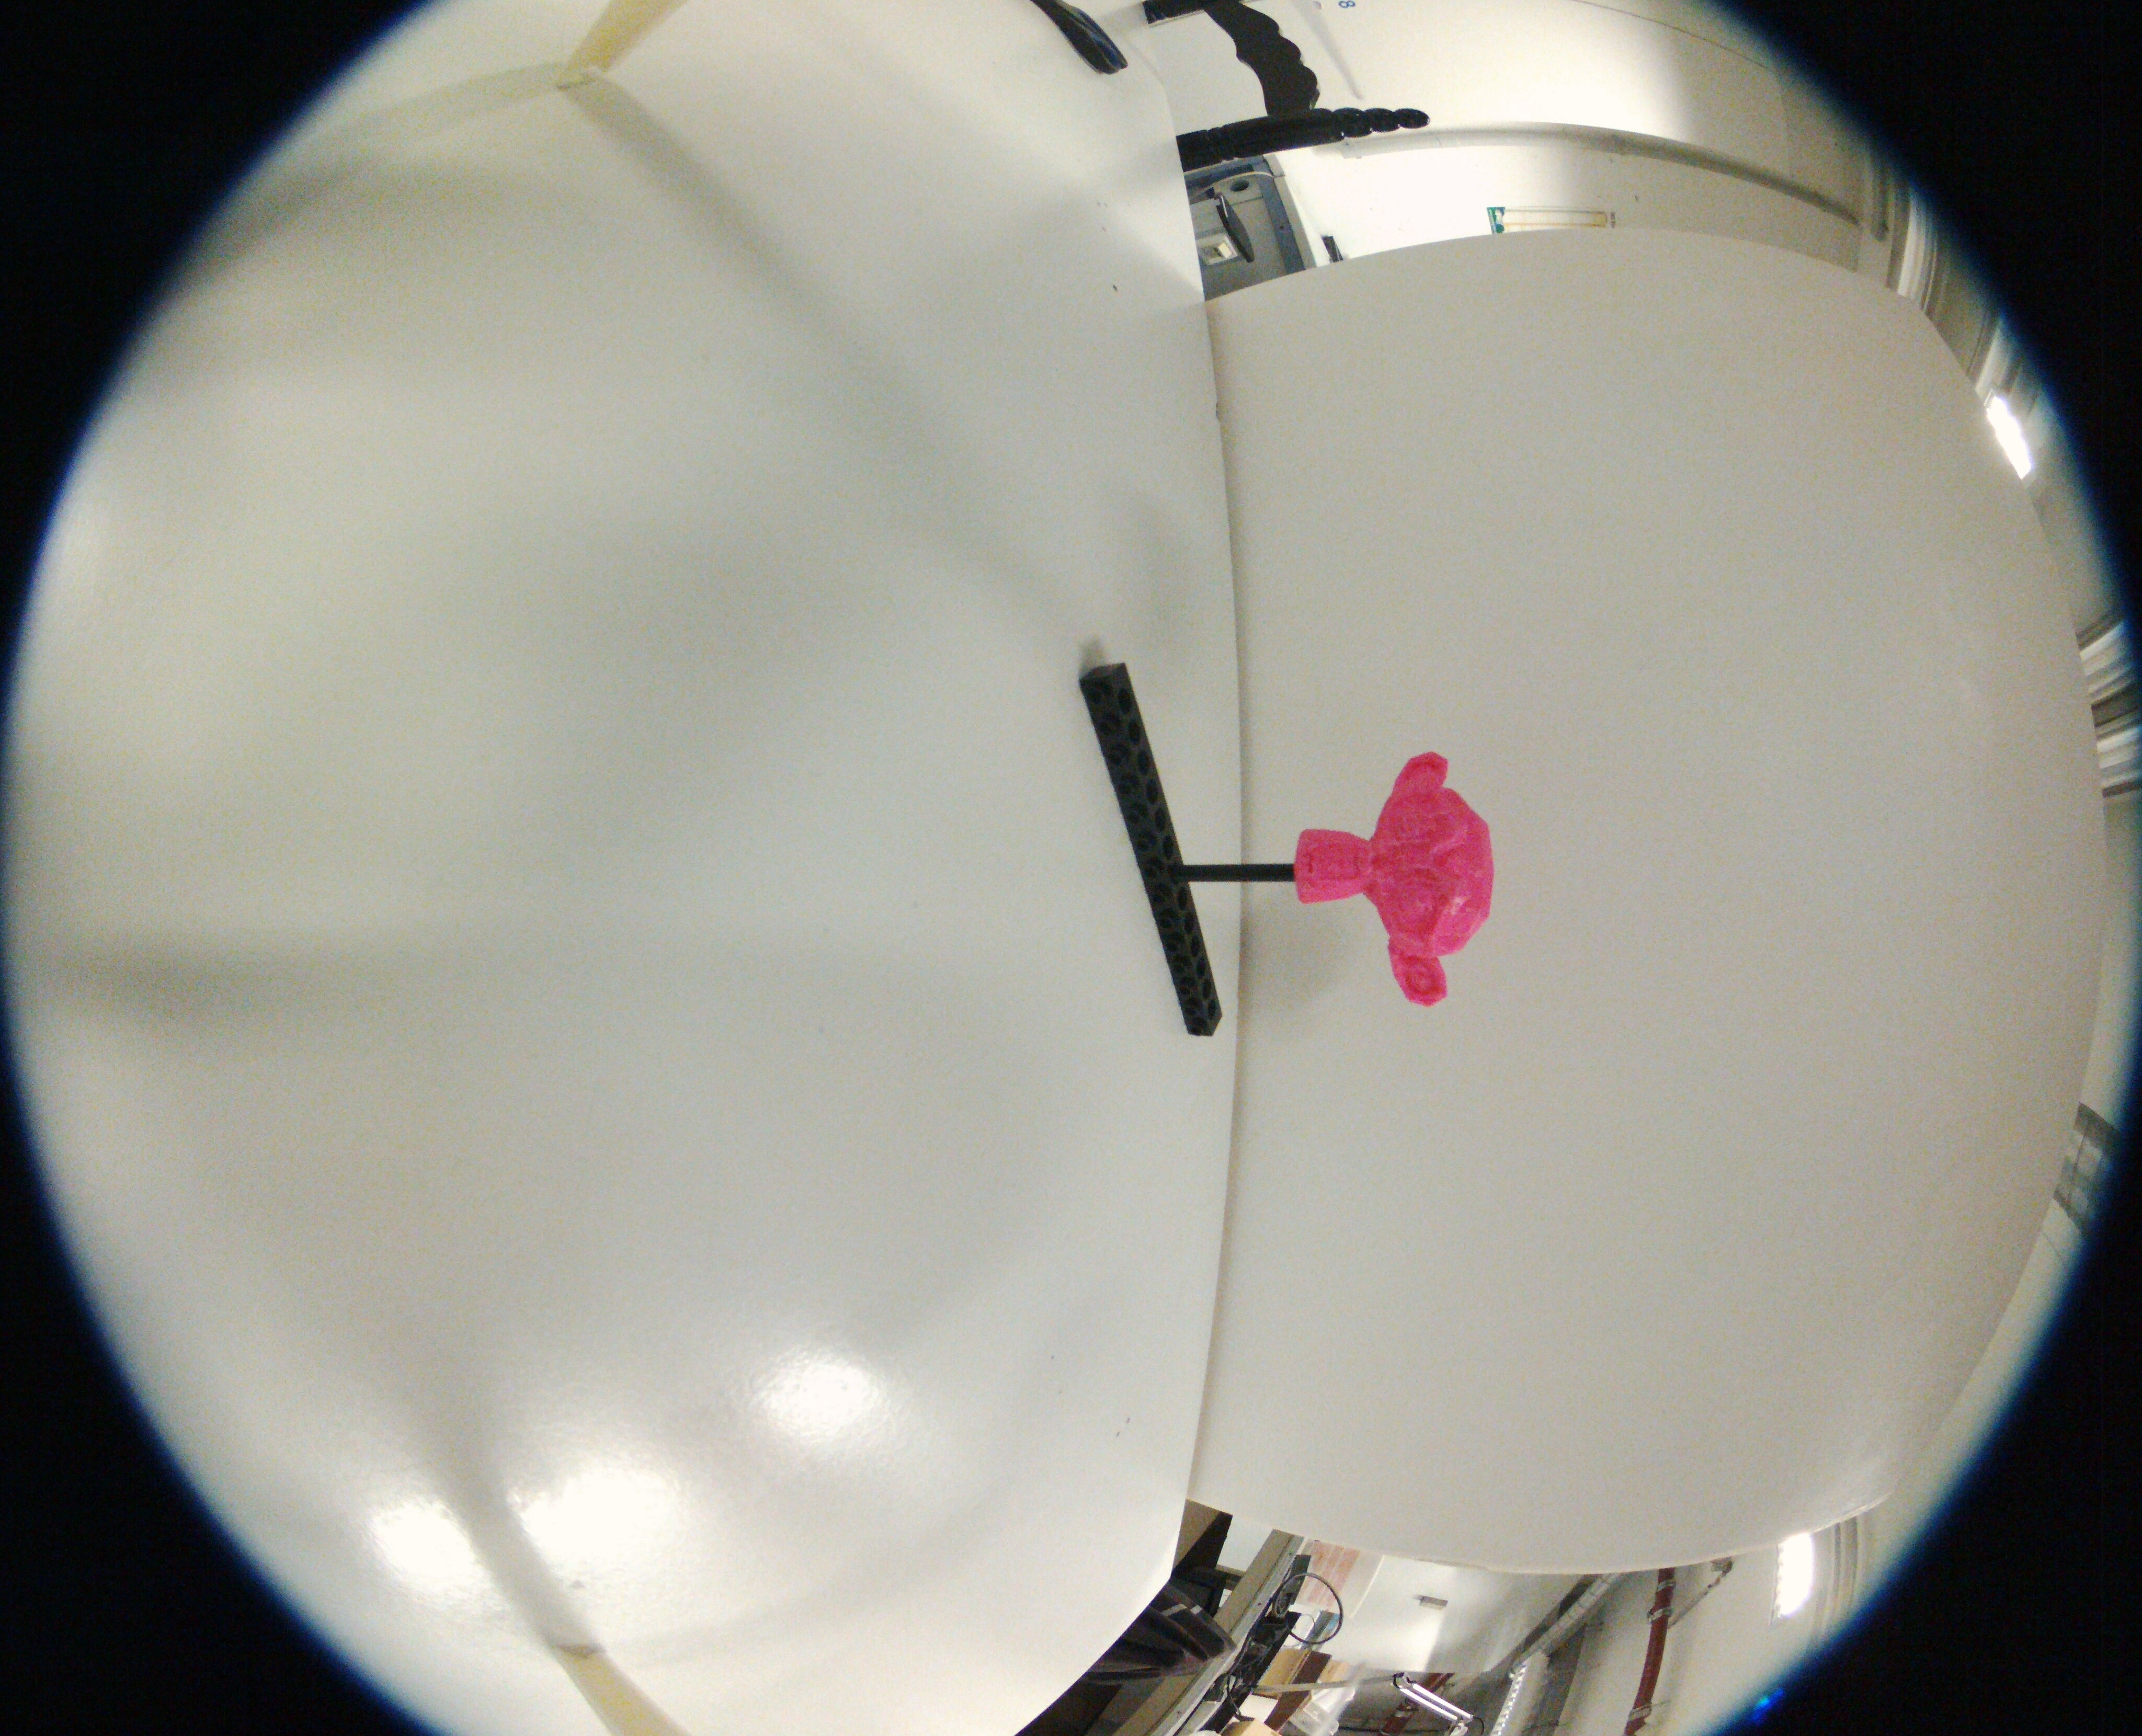
\includegraphics[width=0.48\textwidth]{img/experiment1_original_bebop_img_1.jpg}
		\hfill
		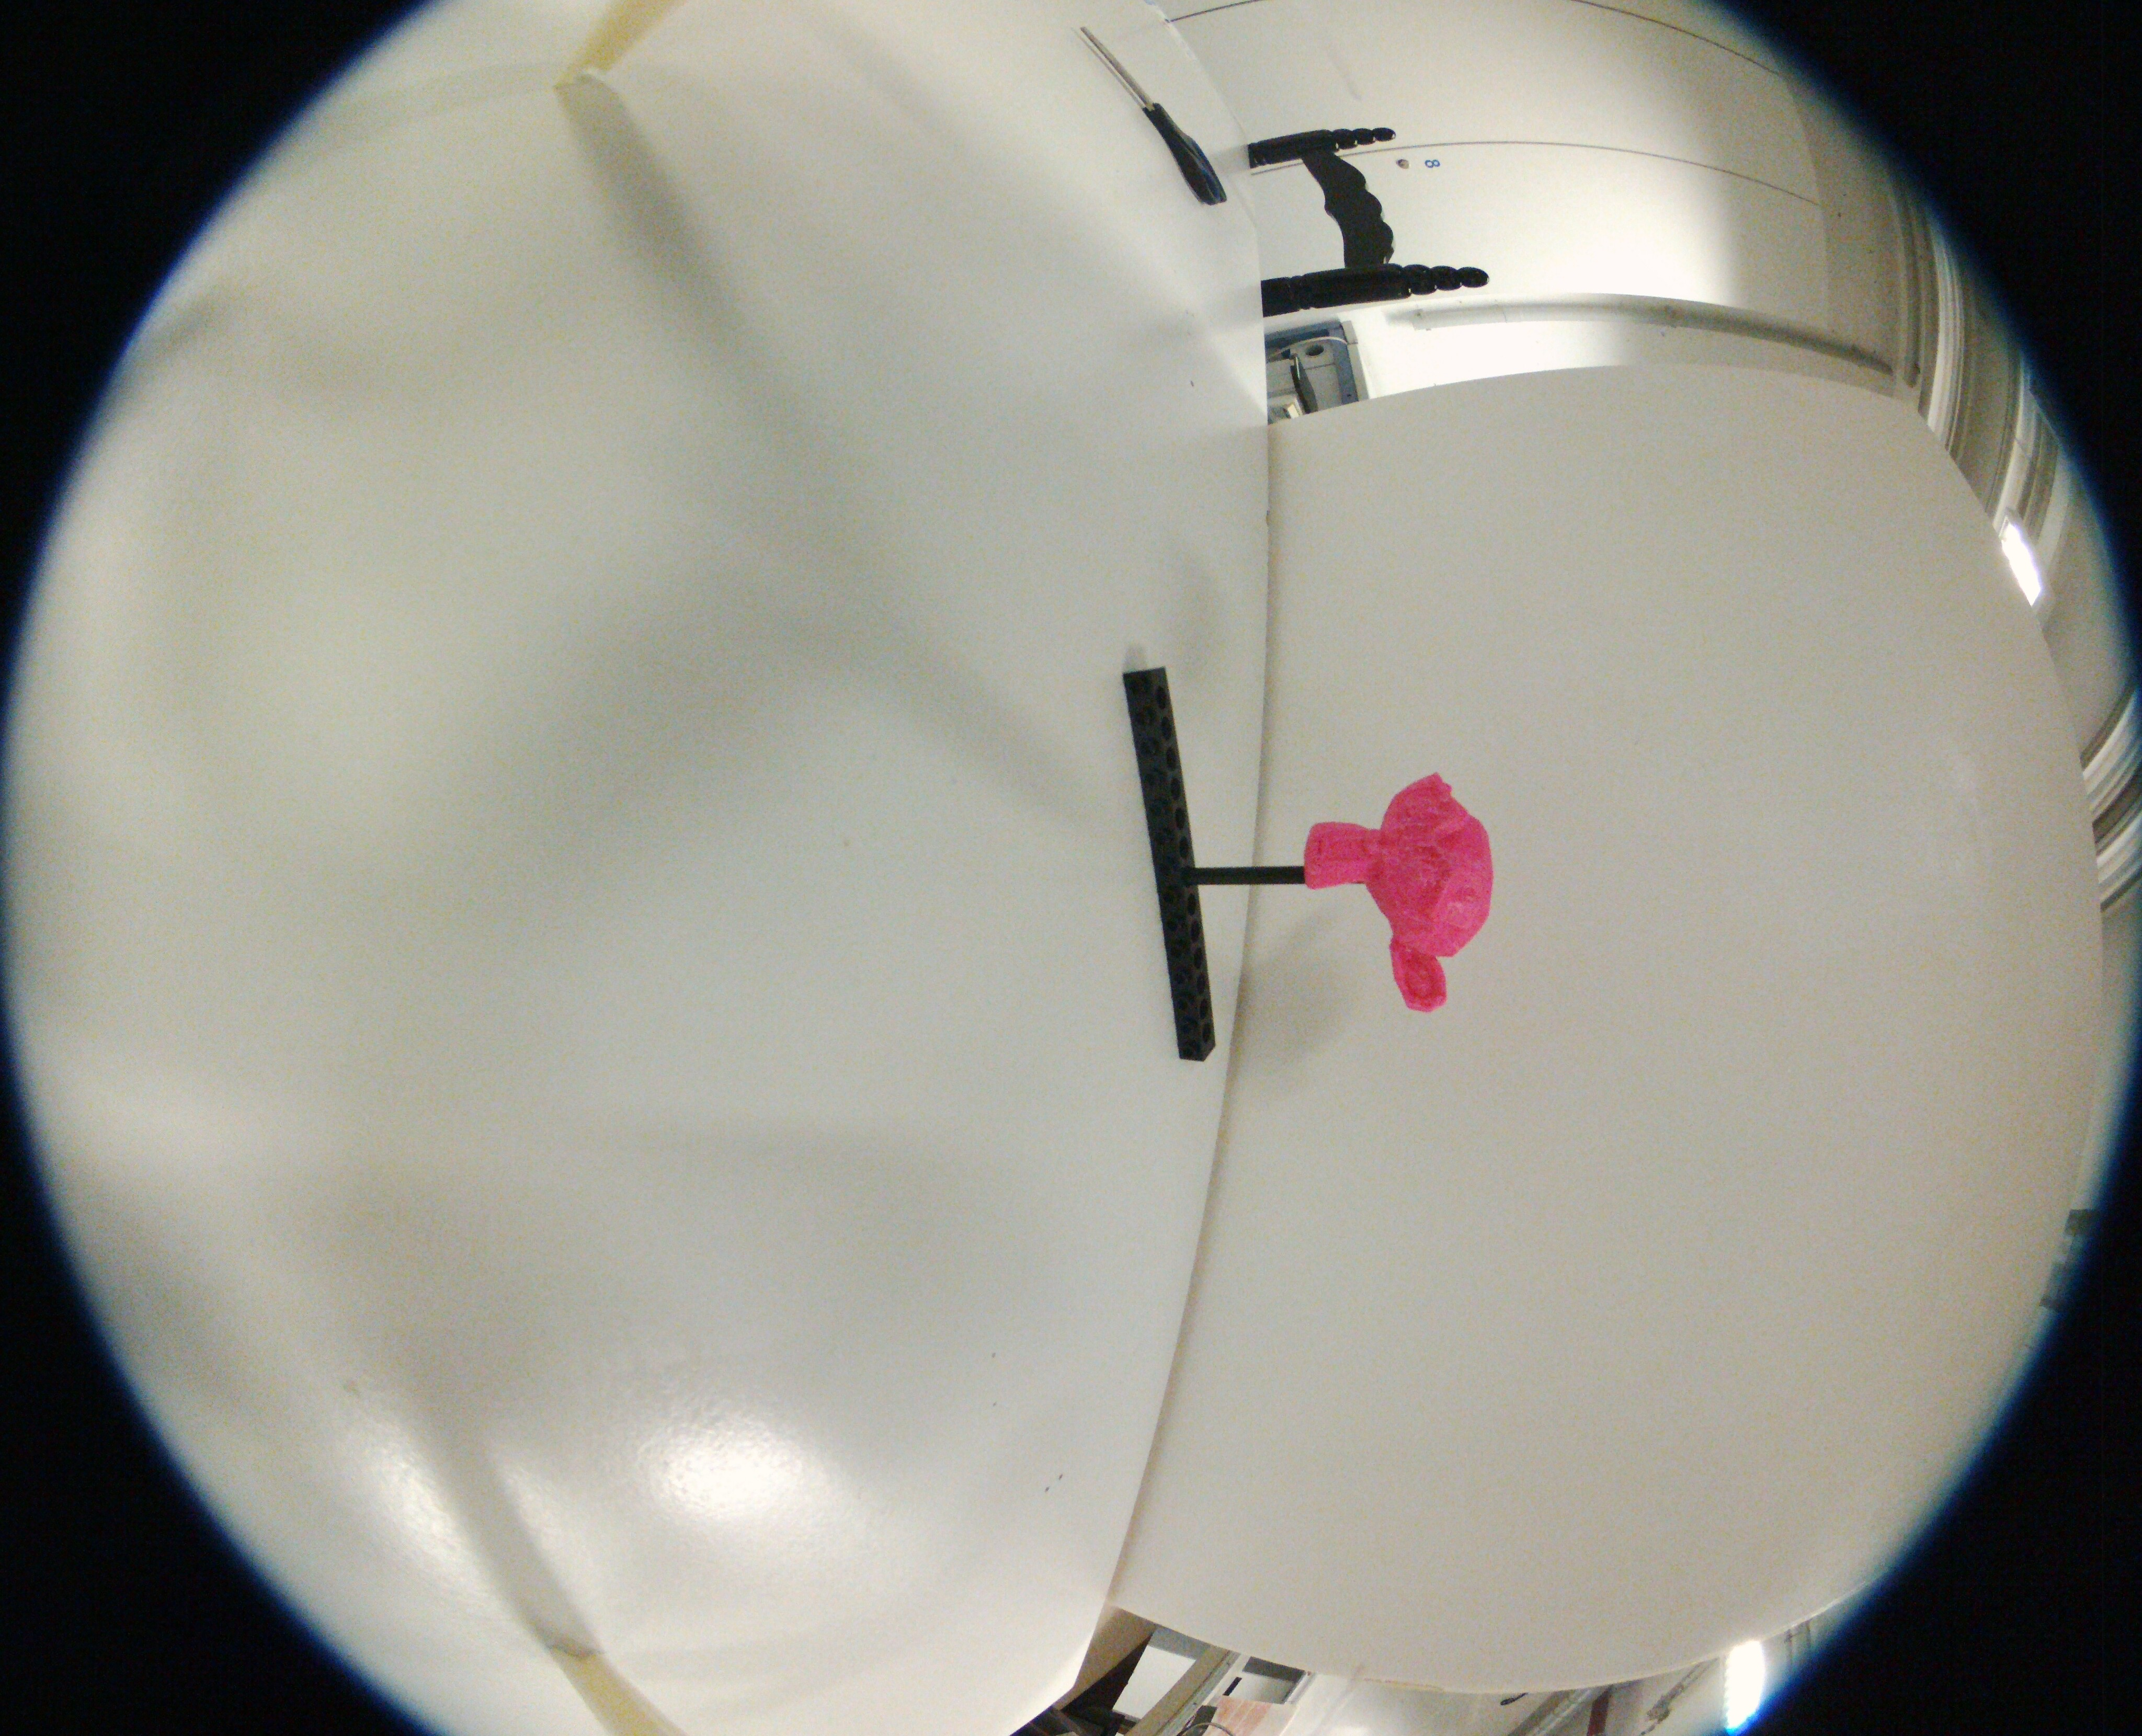
\includegraphics[width=0.48\textwidth]{img/experiment1_original_bebop_img_2.jpg}
		\caption{The original images of the 3D printed monkey head produced by the Parrot~Bebop~2.}
	\end{subfigure}
	~ 
	\begin{subfigure}[t]{\textwidth}
		\centering
		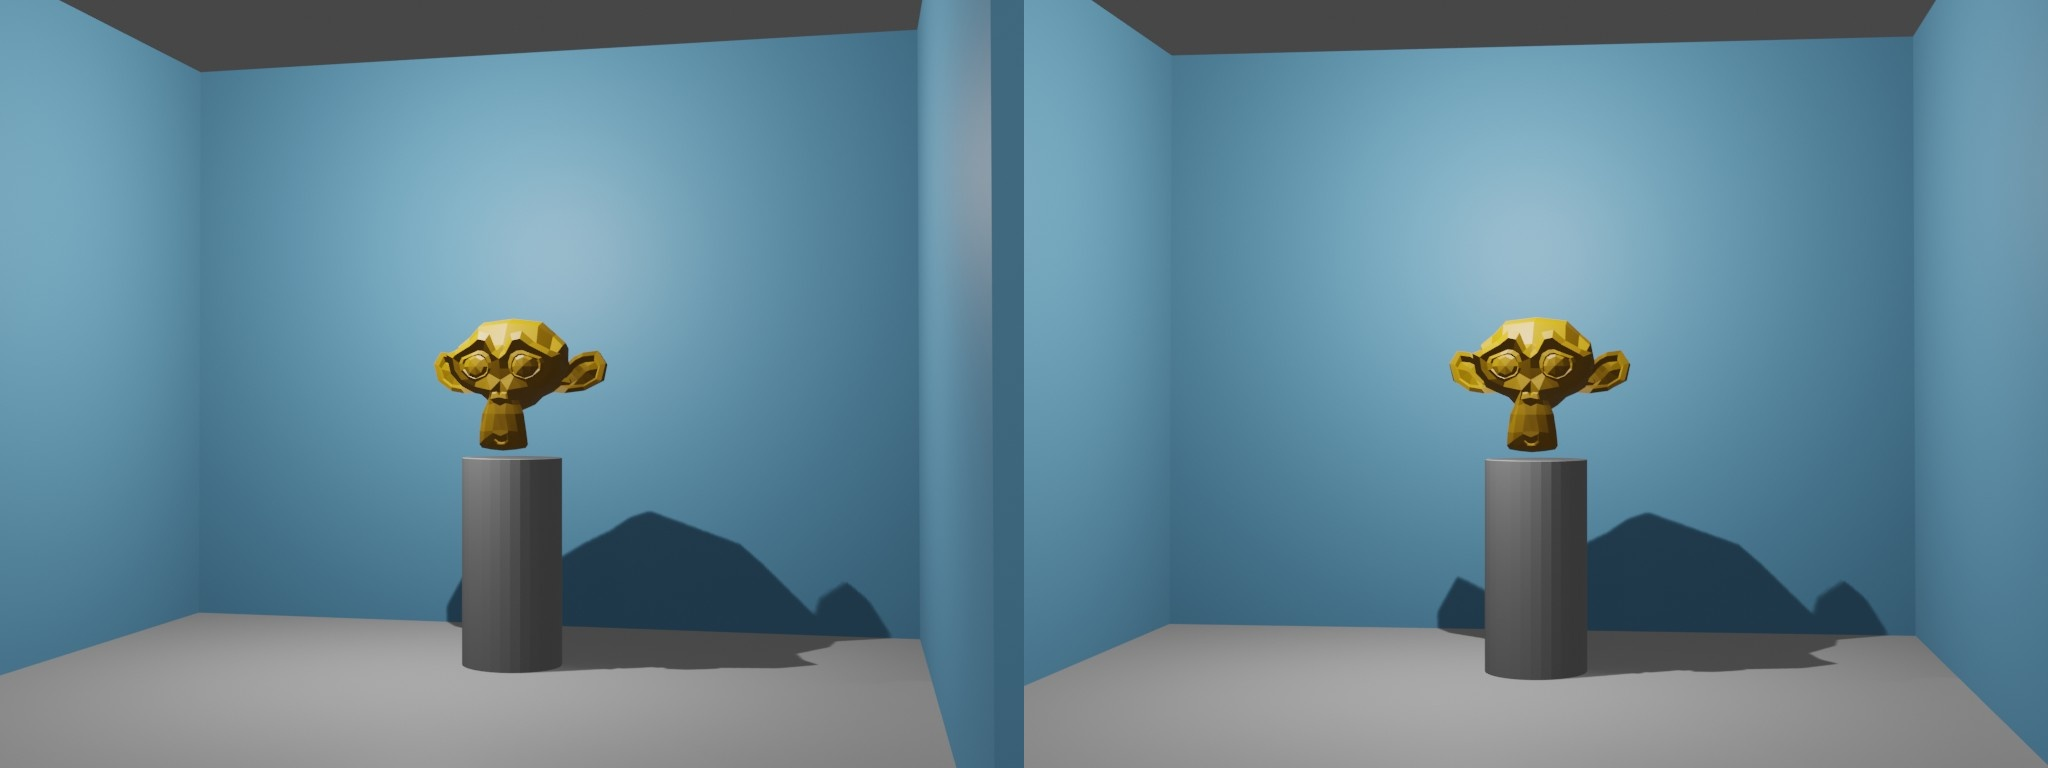
\includegraphics[width=\textwidth]{img/experiment2_environment_comparison_2.jpg}
		\caption{An example training image generated with the help of Blender.}
	\end{subfigure}
	~ 
	\begin{subfigure}[t]{\textwidth}
		\centering
		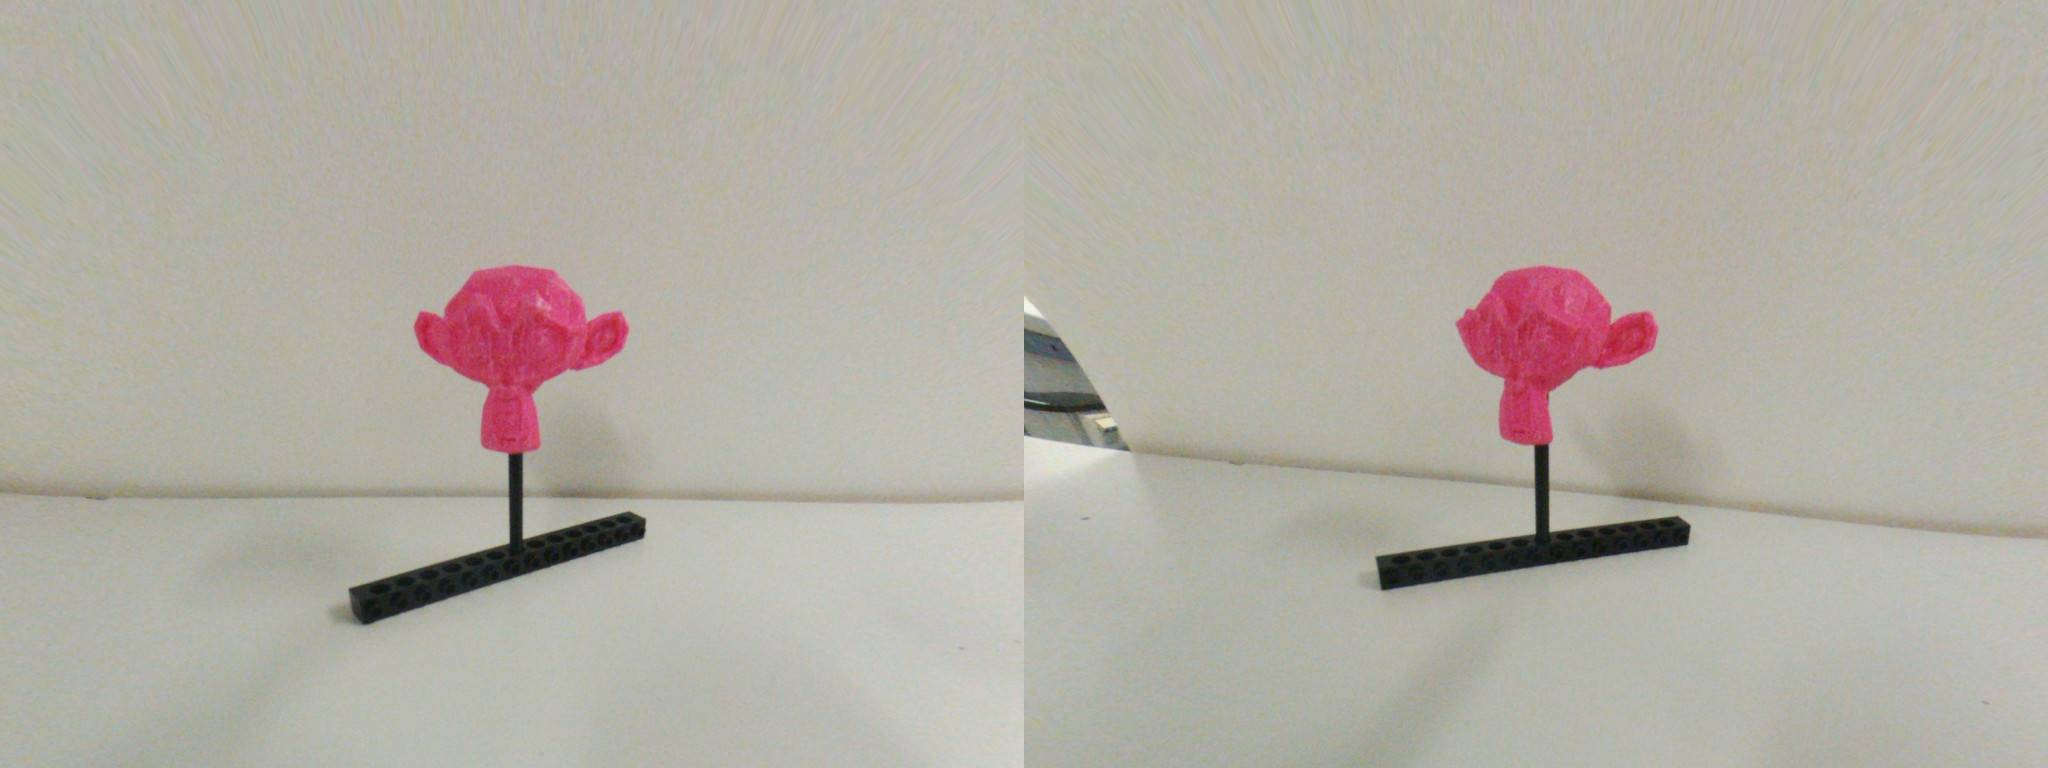
\includegraphics[width=\textwidth]{img/experiment2_environment_comparison_1.jpg}
		\caption{The two modified images of the 3D printed monkey head taken with the Parrot Bebop 2.}
	\end{subfigure}
	\caption{Image pairs of the monkey head.}
	\label{pic:experiment2_environment_comparison}
\end{figure*}


\section{Materials}
[TODO: viele Fotos]

\section{Sequence of Events}

\section{Results}

\filbreak